\documentclass[../main.tex]{subfiles}
\begin{document}
\newpage
\section{Вычисление площадей.}
\emph{Площадь} - неотрицательная функция множества, заданная на некой совокупности множеств \( D(S)\), которые называются \emph{квадрируемыми}. Более полное и подробное определение площади будет дано когда-нибудь позже, когда мы будем разбирать теорию меры, а пока ограничимся этим. \\

{\parindent0pt \textbf{Свойства площади:}}

\begin{enumerate}
    \item \emph{Аддитивность.} Мы привыкли, что площадь аддитивна в том смысле, что если разрезать фигуру на 2 части, то площадь фигуры - это сумма площадей
    обрезков. Но площадь аддитивна ещё и в таком смысле:
    \[ A,B\in D\left( S\right),\quad A \cap B=\varnothing \implies S\left( A \cup B\right)=S\left( A\right)+S\left( B\right)\]
    Это свойство, в частности, позволяет во многих задачах рассматривать площадь как аддитивную функцию промежутка и для её вычисления применять признак плотности. \hyperlink{q15}{Пример можно найти в 15 билете.}
    \item \emph{Инвариантность относительно изометрий (движений).} 
    \[ \Let \;  u: \R^2 \longrightarrow \R^2:\quad  \;\forall \;x,y\in\R^2\quad \left| \left| u\left( x\right)-u\left( y\right)\right|\right|=\left| \left| x-y\right|\right| \implies S\left( u\left( A\right)\right)=S\left( A\right)\]  
    Отображение u, удовлетворяющее условию этого утверждения, называется \hypertarget{def:movement}{\emph{движением}}.
\end{enumerate}

Если \( f \geq 0\), то \( \displaystyle\int\limits_{ a}^{ b}f(x)dx=S\left( \left[ a,b\right],f\right)\) - \emph{площадь подграфика} функции \( f\).

\begin{thm}[Площадь криволинейной трапеции]
    \( \Let \; f,g\in C\left[ a,b\right],\) \[ \forall \;x \in \left[ a,b\right]\; f\left( x\right) \leq g\left( x\right),\quad E = \left\{ \left( x,y\right): \; x \in \left[ a,b\right], \; f\left( x\right) \leq y \leq g\left( x\right)\right\}\]
    Тогда \[ S\left( E\right) = \displaystyle\int\limits_{ a}^{ b} f\left( x\right)-g\left( x\right)dx\]
\end{thm}
\begin{proof}
    
    ~

    \InsertBoxR{0}{
        \begin{minipage}[t]{6cm} 
            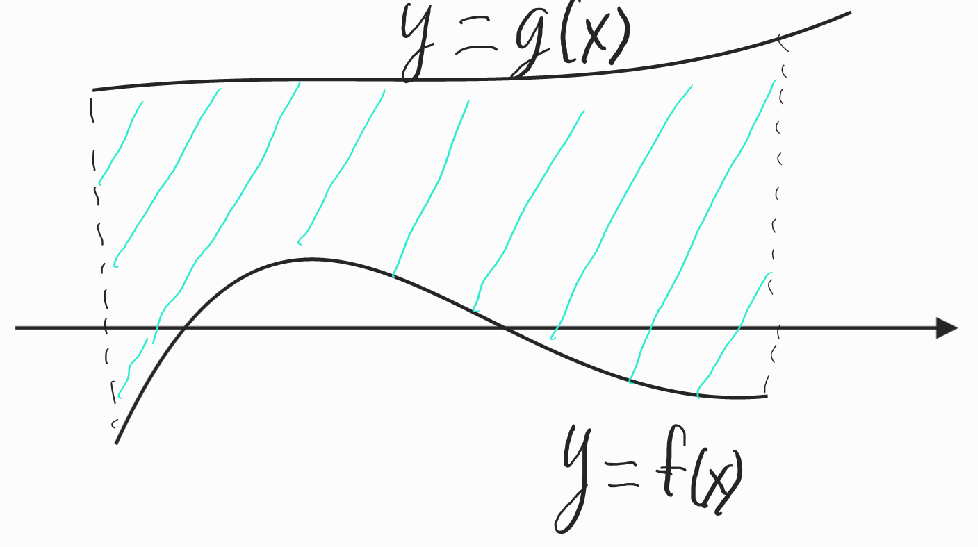
\includegraphics[width=\linewidth]{40_curved.pdf} 
        \end{minipage}
    }
    Этот факт очень простой, если \( f, g \geq 0\), потому что тогда площади их подграфиков - это интегралы, а про них мы всё знаем. Если же \(f\) или \( g < 0\), то мы можем просто передвинуть их так, чтобы на нужном отрезке они 
    обе были \( \geq 0\), а площадь сохранится, т.к. она сохраняется при движении. 
    
    \[ \Let \; m= \min\limits_{ \left[ a,b\right]} f\left( x\right),\quad f_1\left( x\right)=f\left( x\right)-m, \quad f_2\left( x\right)=f\left( x\right)-m\]
    \[ E_1=\left\{ \left( x,y\right):\; f_1\left( x\right) \leq y \leq g_1\left( x\right)\right\}=E+ \left( 0,m\right)\quad\text{-  сдвиг на вектор}\]

    \( S(E_1)=S(E)\), т.к. площадь инвариантна относительно изометрий, в том числе и относительно параллельного переноса. При этом \( f_1 \geq 0,\; g \geq 0\), поэтому
    \[ S\left( E\right)=S\left( \left[ a,b\right],g_1\right)-S\left( \left[ a,b\right],f_1\right)= \displaystyle\int\limits_{ a}^{ b} \left( g\left( x\right)-m\right)dx- \displaystyle\int\limits_{ a}^{ b} \left( f\left( x\right)-m\right)dx= \displaystyle\int\limits_{ a}^{ b} g\left( x\right)-f\left( x\right)dx\]
\end{proof}

\newpage
\begin{example}[\hypertarget{thm:elips_area}{Площадь эллипса}]

    ~

    \InsertBoxR{0}{
        \begin{minipage}[t]{6cm} 
            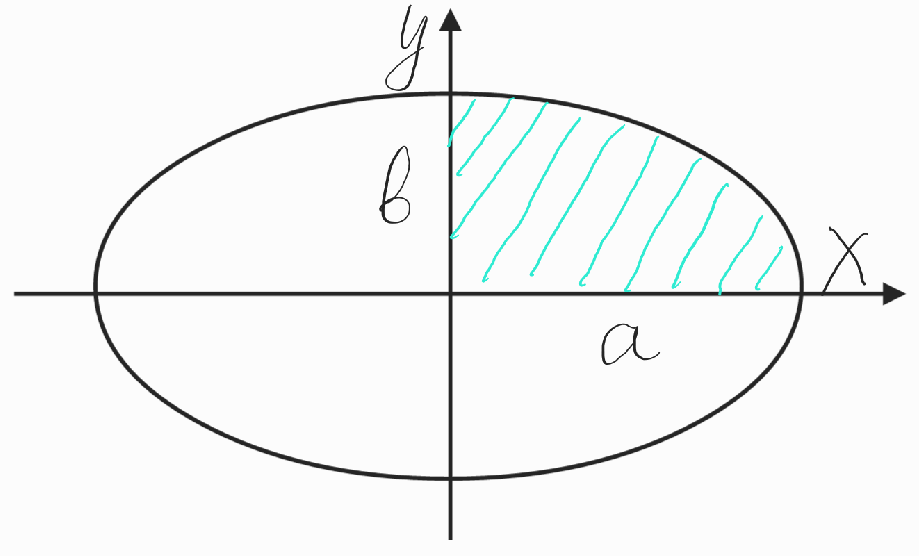
\includegraphics[width=\linewidth]{40_elips.pdf} 
        \end{minipage}
    }
    Вообще, эллипс - это кривая, но здесь речь идёт про площадь множества, ограниченного ей. Если \( a, b\) - полуоси эллипса, то найдём площадь множества 
    \[ E = \left\{ \dfrac{ x^2}{ a^2}+ \dfrac{ y^2}{ b^2} \leq 1\right\}\]

    Т.к. эллипс делится осями координат на 4 симметричные части, будем считать часть одной из них (заштрихованной), а ответ получим умножением на 4. 
    \[ S\left( E\right)=4\left( E \cap \left\{ x \geq 0, \;y \geq 0\right\}\right) = 4S(E_1)\]

    Площадь \(E_1\) будем считать как площадь подграфика функции, заданной уравнением \\
    \( \dfrac{ x^2}{ a^2}+ \dfrac{ y^2}{ b^2}=1\) в первой координатной четверти. 
    \[ y= b\;\sqrt[]{1- \dfrac{ x^2}{ a^2}}\]
    \[ S\left( E_1\right)= \displaystyle\int\limits_{ 0}^{ a} b \;\sqrt[]{1- \dfrac{ x^2}{ a^2}}dx \underset{\tilde{x}= \frac{ x}{ a}}{=} ab\displaystyle\int\limits_{ 0}^{ 1} \sqrt[]{1- \tilde{x}^2}d \tilde{x} \underset{ 
        t=\arcsin{ \tilde{x}}}{=} ab\displaystyle\int\limits_{ 0}^{ \frac{ \pi}{ 2}} \cos^2tdt= \dfrac{ \pi}{ 4}ab\]
    \[ \boxed{S\left( E\right)= \pi ab}\]

    Так мы заодно проверили, что площадь круга равна \( \pi r^2\).
\end{example}

\begin{example}[Площадь криволинейного сектора]
    
    ~

    Криволинейный сектор можно определить как множество точек, ограниченное углом и некоторой кривой - функцией от угла. В полярной системе координат это можно описать как 
    \[ E=\left\{ \left( \varphi , \rho\right): \; \varphi \in \left[ a , b \right],\; 0 \leq \rho \leq r\left( \varphi \right)\right\}\]
    где \( r\left( \varphi \right) \in C\left[ a , b \right]\) - расстояние от начала координат до ограничивающей кривой при угле \( \varphi \).

    \InsertBoxL{0}{
    \begin{minipage}[t]{7cm} 
        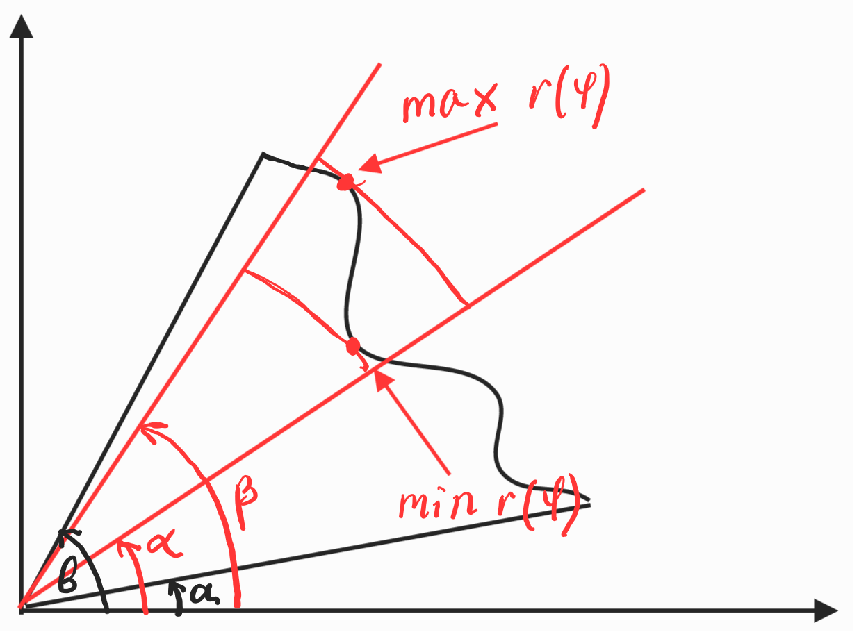
\includegraphics[width=0.98\linewidth]{40_sector.pdf} 
    \end{minipage}
    }   

    Рассмотрим аддитивную функцию промежутка \\
    \( S(\left[ \alpha , \beta \right])\) - площадь части нашего криволинейного сектора, заключённой между 
    углами \( \alpha \) и \( \beta \). Она определена на всех подотрезках отрезка \( \left[ a,b\right]\). Рассмотрим произвольный подотрезок \( \left[ \alpha , \beta \right]\).
    Площадь соответствующей части криволинейного сектора ограничивается снизу вписанным круговым сектором с радиусом, равным \( \min\limits_{ \varphi \in \left[ \alpha , \beta \right]} r\left( \varphi \right)\). 
    Она также ограничивается снизу "описанным"  круговым сектором с радиусом \( \max\limits_{ \varphi \in \left[ \alpha , \beta \right]} r\left( \varphi \right)\). Поэтому мы можем написать:
    \[ \pi \left( \min\limits_{ \varphi \in \left[ \alpha , \beta \right]} r\left( \varphi \right) \right)^2\cdot \dfrac{ \beta-\alpha}{ 2 \pi } \leq S(\left[ \alpha , \beta \right]) \leq \pi \left( \max\limits_{ \varphi \in \left[ \alpha , \beta \right]} r\left( \varphi \right) \right)^2\cdot \dfrac{ \beta-\alpha}{ 2 \pi }\]

    Немного причесав эти неравенства, получим:
    \[ \min\limits_{ \varphi \in \left[ \alpha , \beta \right]} \dfrac{ (r\left(\varphi\right))^2}{ 2}\cdot \left( \beta - \alpha \right) \leq S(\left[ \alpha , \beta \right]) \leq \max\limits_{ \varphi \in \left[ \alpha , \beta \right]} \dfrac{ (r\left(\varphi\right))^2}{ 2}\cdot \left( \beta - \alpha \right)\]

    И так как это верно \( \forall \; \left[ \alpha , \beta \right] \subseteq  \left[ a,b\right]\), \hyperlink{thm:density}{по признаку плотности} \( \dfrac{ (r\left(\varphi\right))^2}{ 2}\) - плотность функции \( S\). Поэтому
    \[ \boxed{ S\left( \left[ a,b\right]\right)= \dfrac{ 1}{ 2}\displaystyle\int\limits_{ a}^{ b}\left( r\left( \varphi \right)\right)^2d \varphi }\]
\end{example}

\begin{example}[Площадь лемнискаты Бернулли]
    
    ~

    \InsertBoxL{0}{
    \begin{minipage}[t]{6cm} 
        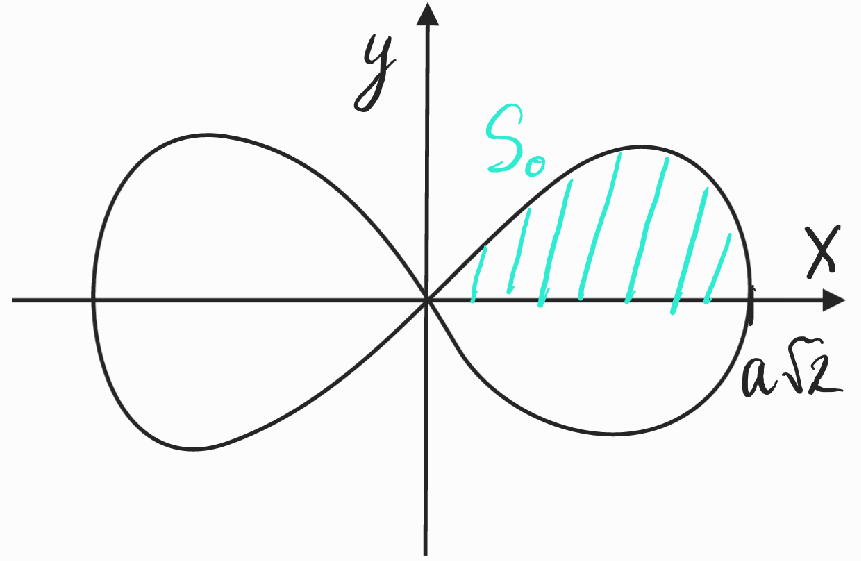
\includegraphics[width=0.98\linewidth]{40_lemniscata.pdf} 
    \end{minipage}
    }   

    Лемниската Бернулли - это кривая, которая в полярных координатах задаётся уравнением \( r = a \;\sqrt[]{2 \cos \left( 2 \varphi \right)}\). 
    Мы хотим найти площадь, которую эта кривая ограничивает. Сначала немного преобразуем равенство:
    \[ r^2 = 2a^2 \cos\left( 2 \varphi \right)\]
    \begin{equation}\label{eq:lemniscata}
        r^4=r^2 \cdot r^2=2a^2\cos\left( 2 \varphi \right)\cdot r^2=2a^2\left( r^2\cos ^2 \varphi - r^2\sin^2 \varphi \right)
    \end{equation}

    Полярная и декартова системы координат связаны друг с другом так: 
    \begin{equation*}
        \begin{cases}
            x=r\cos \varphi \\ 
            y=r\sin \varphi 
        \end{cases}
        \implies 
        \begin{cases}
            r^2\cos^2 \varphi =x^2\\
            r^2\sin^2 \varphi =y^2\\ 
            x^2+y^2=r^2\left( \cos^2 \varphi +\sin^2 \varphi \right)=r^2 \implies r^4=\left( x^2+y^2\right)^2
        \end{cases}
    \end{equation*}

    Подставим это в равенство \ref{eq:lemniscata}, получим: 
    \[ (x^2+y^2)^2=2a^2\left( x^2-y^2\right)\]

    Из этого уравнения видно, что кривая симметрична относительно осей \( x\) и \( y\) (если поставить \( -x\) вместо \( x\) или \( -y\) вместо \( y\) будет то же самое). Поэтому мы будем искать площадь \( S_0\) только той части кривой, которая 
    лежит в первой координатной четверти, то есть там где \( \varphi \in \left[ 0, \dfrac{ \pi}{ 2}\right]\), а потом умножим её на 4 и получим полную площадь \( S\).
    \begin{equation*}
        \begin{cases}
            \varphi \in \left[ 0, \dfrac{ \pi}{ 2}\right]\\
            \cos 2 \varphi \geq 0
        \end{cases}
        \implies 
        \varphi \in \left[ 0, \dfrac{ \pi}{ 4}\right]
    \end{equation*}

    У нас есть промежуток, в пределах которого меняется угол \( \varphi \), есть функция \( r\left( \varphi \right)\), которая задаёт кривую. Значит
    для расчёта площади мы можем использовать формулу площади криволинейного сектора. 

    \[ S_0= \dfrac{ 1}{ 2} \displaystyle\int\limits_{ 0}^{ \frac{ \pi}{ 4}} 2a^2\cos\left( 2 \varphi \right)d \varphi =a^2 \displaystyle\int\limits_{ 0}^{ \frac{ \pi}{ 4}} \cos \left( 2 \varphi \right)d \varphi = a^2\left( \dfrac{ 1}{ 2} \sin\left( 2 \varphi \right)|_{0}^{\frac{ \pi}{ 4}}\right) = \dfrac{ a^2}{ 2}\]

    \[ \boxed{S=2a^2}\]
\end{example}
\end{document}